% Generated in part using
% https://github.com/numpde/ibiocomp/blob/main/code/20201229_LogicalTables/PlayerA.py

% and
	
% https://crcit.net/c/205b0db18f954c4585b3f87d69fced6c
% https://crcit.net/c/84159c89986c4330978603aeace14aa1

% RA, 2020-12-30
	
\begin{table}[hpbt]
\centering

\begin{minipage}{0.3\linewidth}
	\centering
			
	Winning strategy:
	
	{\ }
	
	\begin{tabular}{cccc|c}
		\multicolumn{4}{c|}{Sticks left} & Take \\
		\hline
		15 & 11 & 7 & 3 & 2 \\
		14 & 10 & 6 & 2 & 1 \\	
		13 & 9  & 5 & 1 & 1 \\	
		12 & 8  & 4 &   & 3 \\	
	\end{tabular}
\end{minipage}
%
\qquad
%
\begin{minipage}{0.25\linewidth}
	\centering
	\begin{tabular}{ccc|cc}
		\ce{w_A} &  \ce{s_1} &  \ce{s_0} &  \ce{r_1} &  \ce{r_0} \\
		\hline
		 0 &   0 &   0 &   0 &   0 \\
		 0 &   0 &   1 &   0 &   0 \\
		 0 &   1 &   0 &   0 &   0 \\
		 0 &   1 &   1 &   0 &   0 \\
		 1 &   0 &   0 &   1 &   1 \\
		 1 &   0 &   1 &   0 &   1 \\
		 1 &   1 &   0 &   0 &   1 \\
		 1 &   1 &   1 &   1 &   0 \\
	\end{tabular}
\end{minipage}
%
\qquad
%
\begin{minipage}{0.25\textwidth}
	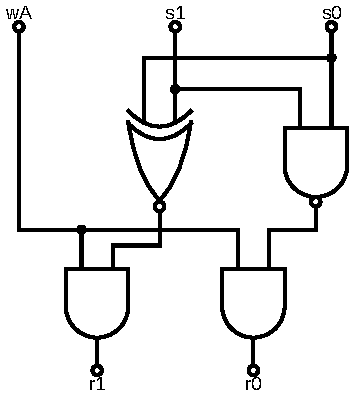
\includegraphics[width=\linewidth]{circuits/Logical-PlayerA.svg.pdf}
\end{minipage}

\caption{%
    Both players follow the same strategy shown.
    %
	The truth table and the logical circuit 
	for Player A
	is shown.
	%
	The input is a
	wake-up signal \ce{w_A}
	and the bits
	\ce{s_1}/\ce{s_0}
	of the current number of sticks
	(\ce{8 s_3 + 4 s_2 + 2 s_1 + s_0}).
	%
	The output is
	the number of sticks taken,
	encoded as \ce{2 r_1 + r_0}.
	%
	The output is cut off when \ce{w_A} is absent.
	%
	%
	The circuit for {Player B}
	is identical except
	that 
	the output is controlled by \ce{w_B}.
}

\label{t:logical-playera}
\end{table}
